% WACV 2027 submission — Paper B (zero-shot cross-script transfer)
\documentclass[10pt,twocolumn,letterpaper]{article}

%%%%%%%%% PAPER TYPE  - PLEASE UPDATE FOR FINAL VERSION
\usepackage[review,datasets]{wacv}        % REVIEW version, Evaluations & Datasets track
% \usepackage{wacv}              % camera-ready
%\usepackage[pagenumbers]{wacv} % arXiv version

\input{preamble}
% ---------------------------------------------------------------------------
% numbers.tex — single source for every campaign number quoted in the paper.
% Values are re-derived from the result JSONs by verify_wacv_numbers.py; run it
% before every submission build and diff against this file.
% ---------------------------------------------------------------------------

% ---- Rung A (source-only baseline) WRR, % ----
\newcommand{\wrrAtamil}{0.0}
\newcommand{\wrrAtelugu}{1.28}
\newcommand{\wrrAkannada}{2.78}
\newcommand{\wrrAmalayalam}{0.18}
\newcommand{\wrrAoriya}{0.77}
\newcommand{\wrrAgujarati}{3.05}
\newcommand{\wrrAbengali}{1.39}
\newcommand{\wrrAdevanagari}{5.46}
\newcommand{\wrrAgurmukhi}{0.59}

% ---- Rung B (+ synthetic target, zero real) WRR, % ----
\newcommand{\wrrBtamil}{9.16}
\newcommand{\wrrBtelugu}{19.82}
\newcommand{\wrrBkannada}{15.42}
\newcommand{\wrrBmalayalam}{9.69}
\newcommand{\wrrBoriya}{25.38}
\newcommand{\wrrBgujarati}{15.86}
\newcommand{\wrrBbengali}{27.08}
\newcommand{\wrrBdevanagari}{30.09}
\newcommand{\wrrBgurmukhi}{22.16}
\newcommand{\wrrBmin}{9.16}
\newcommand{\wrrBmax}{30.09}

% ---- Rung B character accuracy (1 - CER), % ----
\newcommand{\chaBtamil}{39.0}
\newcommand{\chaBtelugu}{54.43}
\newcommand{\chaBkannada}{46.37}
\newcommand{\chaBmalayalam}{34.57}
\newcommand{\chaBoriya}{56.37}
\newcommand{\chaBgujarati}{38.49}
\newcommand{\chaBbengali}{57.77}
\newcommand{\chaBdevanagari}{57.16}
\newcommand{\chaBgurmukhi}{44.1}

% ---- test-set sizes ----
\newcommand{\ntamil}{513}\newcommand{\ntelugu}{545}\newcommand{\nkannada}{720}
\newcommand{\nmalayalam}{547}\newcommand{\noriya}{1044}\newcommand{\ngujarati}{1015}
\newcommand{\nbengali}{2873}\newcommand{\ndevanagari}{6042}\newcommand{\ngurmukhi}{2879}

% ---- Rung Bbpe (stock-BPE ablation) WRR, % — 9/9 complete 2026-07-19 ----
\newcommand{\wrrPtamil}{2.34}
\newcommand{\wrrPtelugu}{10.28}
\newcommand{\wrrPkannada}{13.33}
\newcommand{\wrrPmalayalam}{4.2}
\newcommand{\wrrPoriya}{14.94}
\newcommand{\wrrPgujarati}{13.69}
\newcommand{\wrrPbengali}{19.07}
\newcommand{\wrrPdevanagari}{27.99}
\newcommand{\wrrPgurmukhi}{17.65}
\newcommand{\chaPtamil}{30.45}
\newcommand{\chaPtelugu}{55.1}
\newcommand{\chaPkannada}{48.76}
\newcommand{\chaPmalayalam}{31.16}
\newcommand{\chaPoriya}{50.64}
\newcommand{\chaPgujarati}{37.18}
\newcommand{\chaPbengali}{52.67}
\newcommand{\chaPdevanagari}{58.72}
\newcommand{\chaPgurmukhi}{43.42}
% ---- ablation summary statistics (all nine scripts) ----
\newcommand{\bpeRatioMin}{1.08}       % Devanagari: 30.09/27.99
\newcommand{\bpeRatioMax}{3.91}       % Tamil: 9.16/2.34
\newcommand{\bpeSignP}{0.0039}        % exact two-sided sign test, 9/9 same direction
% exploratory (post hoc, NOT preregistered): fertility vs BPE-penalty ratio B/Bbpe
\newcommand{\spearFertPenalty}{+0.73}     % Spearman(fertility, B/Bbpe), n=9
\newcommand{\spearFertPenaltyP}{0.031}    % exact two-sided permutation p
\newcommand{\spearFertPenaltyDiff}{+0.28} % same on absolute difference B-Bbpe (confound check)

% ---- pivot-space token coverage (result-blind, computed 2026-06-25), % ----
\newcommand{\covgujarati}{97.3}\newcommand{\covdevanagari}{94.3}\newcommand{\covoriya}{92.6}
\newcommand{\covtelugu}{92.3}\newcommand{\covkannada}{90.8}\newcommand{\covgurmukhi}{90.7}
\newcommand{\covtamil}{88.8}\newcommand{\covbengali}{87.3}\newcommand{\covmalayalam}{79.2}

% ---- campaign-level statistics (9 Rung-B points) ----
\newcommand{\spearCovRaw}{+0.37}      % Spearman(token coverage, WRR), all nine
\newcommand{\spearCovEqual}{+0.61}    % among the seven equal-synth (3240) scripts
\newcommand{\spearFert}{-0.80}        % Spearman(fertility, WRR) — preregistered primary, refuted
\newcommand{\spearVissim}{-0.14}      % frozen-encoder visual-similarity control (TODO verify at 9 pts)
% two-factor fit at the 9-point checkpoint: WRR = a + b*tok_cov + c*is2x
\newcommand{\tfIntercept}{-35.79}
\newcommand{\tfCovCoef}{0.583}
\newcommand{\tfTwoxBonus}{11.48}
\newcommand{\tfRMSE}{4.18}

% ---- prospective predictions (filed, committed and pushed before each run) ----
\newcommand{\predKannada}{{\sim}15}\newcommand{\realKannada}{15.42}
\newcommand{\predGurmukhi}{16.2}
\newcommand{\predGurmukhiOneSig}{[12.2, 20.2]}
\newcommand{\predGurmukhiTwoSig}{[8.2, 24.1]}
\newcommand{\realGurmukhi}{22.16}

% ---- Part-1 law (12 balanced-budget runs, N=11 fits) ----
\newcommand{\lawRsqAdv}{0.678}
\newcommand{\lawRsqFusion}{0.698}
\newcommand{\lawLoso}{90.9}
\newcommand{\lawPolarity}{8/9}

% ---- external anchors (different axis: they use real labeled target data) ----
\newcommand{\parseqSynth}{{\sim}47}
\newcommand{\parseqFinetuned}{{\sim}73}
\newcommand{\florenceRawZS}{0.0}
% TODO(vlm): Qwen2.5-VL-7B zero-shot per-script numbers (Amendment 4c)
% TODO(scaling): per-budget WRR for malayalam/kannada/telugu x {810,1620,3240,6480,12960} (4a)
% TODO(khmer): prediction + realized (4b)
   % every campaign number as a macro; regenerated by verify_wacv_numbers.py

\definecolor{wacvblue}{rgb}{0.21,0.49,0.74}
\usepackage[pagebackref,breaklinks,colorlinks,allcolors=wacvblue]{hyperref}

%%%%%%%%% PAPER ID  - PLEASE UPDATE
\def\wacvPaperID{*****}
\def\confName{WACV}
\def\confYear{2027}

%%%%%%%%% TITLE
\title{Reading Unseen Scripts: Predictable Zero-Real-Image Transfer\\for Brahmic Scene Text Recognition}

\author{Anonymous WACV 2027 submission\\Paper ID \wacvPaperID}

\begin{document}
\maketitle
\begin{abstract}
Scene-text recognition (STR) is effectively solved for Latin script yet fails for most of the
world's writing systems, and collecting labeled real images for every script is not a scalable
answer. We ask a stronger question: can a recognizer read a script for which \emph{no real labeled
image exists at all} --- and can its accuracy be \emph{predicted before training}? We construct a
shared grapheme pivot space spanning nine Brahmic scripts and fine-tune a compact open
vision--language model in it under a leave-one-script-out protocol: the held-out script is seen
only as rendered synthetic images, never as a real photograph. On real scene-text benchmarks the
held-out scripts reach \wrrBmin--\wrrBmax\% word recognition (character accuracy up to
\chaBbengali\%), against source-only baselines of \wrrAtamil--\wrrAdevanagari\%. A prompted
frontier VLM (Qwen2.5-VL-7B), scored with every generosity --- its prose answers parsed in its
favor --- reads only Bengali and Devanagari with any competence
(\vlmWrrBengali/\vlmWrrDevanagari\% WRR) and stays at or near zero on six of the remaining seven
scripts (at most \vlmWrrTamil\%, on Tamil); our compact pivot model wins on \vlmScriptsWon\ of
nine, the VLM leading only on Devanagari, so scale alone does not close the gap. Replacing the
grapheme pivot with the stock BPE tokenizer degrades word recognition on all nine scripts
($\bpeRatioMin\times$--$\bpeRatioMax\times$; exact sign test $p=\bpeSignP$), on three of them
despite equal-or-better character accuracy --- the pivot, not fine-tuning alone, converts
character evidence into word reads. The campaign ran under a frozen preregistration: our primary
hypothesis --- that tokenizer fertility predicts which scripts transfer --- was \emph{falsified}
(Spearman $\spearFert$) and reported as such. A prospectively filed dose--response study then shows
word recognition is \emph{log-linear in synthetic exposure with a script-invariant slope}
($\scaleSlope$ WRR per doubling, $R^2$ up to \scaleRtwoMax); the pre-committed slope
\emph{magnitude} missed by $\scaleSlopeRatio\times$ and is reported as the miss it is. We
deliberately do not claim typology as the driver: pivot-space coverage orders the swept scripts
in-sample but does not generalize to held-out scripts ($r=\covOOSr$), which we disclose. We release
the pivot construction, rendering pipeline, and the zero-real-image evaluation protocol.
\end{abstract}

\section{Introduction}
\label{sec:intro}

Modern scene-text recognizers exceed 90\% word accuracy on Latin benchmarks, yet most of the
world's writing systems remain unreadable to them. Recent audits are stark: across more than a
hundred Unicode scripts, even frontier vision--language models (VLMs) read fewer than thirty, and
on unfamiliar scripts they emit garbled or substituted output~\cite{glotocr}. For the Brahmic
family --- nine major scripts used by over a billion people --- real-image training data exists
only because of recent, labor-intensive benchmark efforts~\cite{indicstr12,bstd}, and dozens of
related scripts (Sinhala, Khmer, Myanmar, Tibetan, \dots) have little or none. Collecting and
annotating real photographs script-by-script is not a scalable path to coverage.

This paper asks a stronger question than ``how well can script $X$ be read with its training
set'': \emph{can a recognizer read a script for which no real labeled image exists at all --- and
can we predict, before training, how well?} We answer both, for scene text, at the granularity of
an entire writing system.

Our approach rests on a structural observation about Brahmic scripts: they descend from a common
ancestor and share an organizational scheme --- consonant bases, vowel signs, and conjunct
formation via a virama --- even though their glyphs and Unicode blocks are disjoint. We exploit
this by constructing a \emph{shared grapheme pivot space}: every script's text is decomposed into
grapheme clusters and mapped by structural correspondence into a common output vocabulary, so that
nine visually unrelated scripts write into one label space. A compact open VLM
(Florence-2, 0.23B parameters~\cite{florence2}) is fine-tuned in this space on real images of
\emph{source} scripts plus rendered \emph{synthetic} images of the target script --- never a real
target photograph.

We evaluate with a leave-one-script-out (LOSO) protocol over all nine scripts of a public
real-image benchmark~\cite{bstd}. For each held-out script we train two models: a source-only
model (Rung~A), and a source+synthetic-target model (Rung~B); both are evaluated on the held-out
script's \emph{real} test images. Transfer is substantial and universal: every script improves
from a \wrrAtamil--\wrrAdevanagari\% baseline to \wrrBmin--\wrrBmax\% word recognition rate
(WRR), with character accuracy up to \chaBbengali\% --- using zero real target images. An
ablation that swaps the grapheme pivot for the stock BPE tokenizer, all else identical, degrades
transfer on all nine scripts ($\bpeRatioMin\times$--$\bpeRatioMax\times$; exact sign test
$p=\bpeSignP$);
strikingly, on Telugu the BPE model matches the pivot model's \emph{character} accuracy
(\chaPtelugu\% vs.\ \chaBtelugu\%) while halving \emph{word} accuracy --- the pivot is what
converts character evidence into whole-word reads.

The second contribution is epistemic, and to our knowledge unprecedented in text recognition: the
campaign was run under a frozen, version-controlled preregistration with an append-only amendment
log, and its predictions were filed \emph{prospectively} --- committed and pushed before the runs
they predict. This cuts both ways, and we report both edges. Our preregistered primary hypothesis
--- that tokenizer \emph{fertility}, the property that governs the supervised grapheme-vs-BPE
trade-off (Sec.~\ref{sec:method}), also predicts which scripts transfer --- was \emph{falsified}
(Spearman $\spearFert$ across nine scripts). What survived is a scaling account: synthetic-exposure
\emph{budget} dominates, and its effect is a \emph{script-invariant, log-linear} dose--response
($\scaleSlope$ WRR per doubling, common-slope $F$-test $p=\scaleFp$; the pre-committed slope
\emph{magnitude} missed by $\scaleSlopeRatio\times$ and is scored as such). We do \emph{not} claim
typology as the driver: pivot-space coverage orders the swept scripts in-sample but does not
generalize out-of-sample ($r=\covOOSr$ across the six held-out scripts), which we disclose rather
than lean on. The forecasting record is auditable: a point forecast of $\predKannada$ WRR for
Kannada (realized \realKannada); a final-script forecast for Gurmukhi of \predGurmukhi\ WRR with
$\pm2\sigma$ band \predGurmukhiTwoSig, filed and pushed 3.7 hours before training began (realized
\realGurmukhi: outer band hit, point under-called --- reported as the miss it is).

\medskip\noindent Our contributions:
\begin{enumerate}
  \item \textbf{Zero-real-image cross-script transfer --- and scale is not the shortcut.} The
  first demonstration, to our knowledge, that real scene text of an entirely unseen script ---
  disjoint Unicode block, disjoint glyph inventory --- can be read by transferring through a
  designed structural pivot space, evaluated LOSO across nine Brahmic scripts
  (\wrrBmin--\wrrBmax\% WRR from ${\le}\,\wrrAdevanagari\%$ baselines). A prompted 7B frontier VLM,
  scored with every generosity, reads only the two highest-resource scripts and loses to our
  compact model on \vlmScriptsWon\ of nine --- the problem is not solved by scale.
  \item \textbf{The pivot is the mechanism.} A preregistered stock-BPE ablation under identical
  data, seed, and recipe degrades WRR on all nine scripts
  ($\bpeRatioMin\times$--$\bpeRatioMax\times$; exact sign test $p=\bpeSignP$), isolating
  \emph{output-space structure} --- not synthetic fine-tuning per se --- as the transfer
  mechanism; exploratorily, the size of the penalty tracks the script's fertility
  (Sec.~\ref{sec:fertility-fails}).
  \item \textbf{Predictability, tested prospectively --- audited both ways.} A frozen,
  version-controlled preregistration with committed-before-run forecasts. The preregistered primary
  (fertility predicts transfer) was \emph{falsified} (Spearman $\spearFert$) and reported in full.
  A prospectively filed synthetic-scaling study establishes a \emph{script-invariant, log-linear}
  dose--response (slope $\scaleSlope$ WRR/doubling, common-slope $F$-test $p=\scaleFp$); the
  pre-committed slope magnitude missed by $\scaleSlopeRatio\times$ and is scored as a miss. We
  decline the typology-as-driver claim: pivot coverage orders scripts in-sample but does not
  generalize out-of-sample ($r=\covOOSr$), disclosed rather than buried
  (Sec.~\ref{sec:experiments}).
  \item \textbf{Artifacts.} The pivot construction, rendering and verification pipeline,
  evaluation protocol, and the preregistration/prediction chain itself, released as a reusable
  template for prospective empirical ML.
\end{enumerate}

We do not claim per-script state of the art: supervised recognizers trained on real labeled
target images reach ${\sim}73\%$ on this benchmark~\cite{bstd} and sit on a different axis ---
they presuppose the data whose absence defines our problem. The relevant comparisons, which we
report, are source-only baselines, the BPE ablation, raw and frontier VLMs on the same test sets,
and our own prospective forecasts.

\section{Related Work}
\label{sec:related}

\paragraph{Multilingual STR and Indic benchmarks.}
STR is mature for Latin script~\cite{parseq}, but coverage collapses elsewhere.
IndicSTR12~\cite{indicstr12} and the Bharat Scene Text Dataset~\cite{bstd} established real-image
benchmarks for Indian languages; on the latter, PARSeq reaches $\parseqSynth\%$ average WRR
trained on synthetic data only and $\parseqFinetuned\%$ after fine-tuning on real labeled images
--- numbers that presuppose labeled target data. GlotOCR~\cite{glotocr} quantifies the wider
problem: frontier VLMs read fewer than thirty of 100+ scripts. Synthetic-data engines for STR
remain Latin-centric~\cite{unionst}, and fine-tuning VLMs on synthetic renderings has been shown
for a single low-resource script with real-data validation~\cite{manchu}. Our work targets the
regime where no real labeled target image exists, and asks not only whether such scripts can be
read but how well, predicted in advance.

\paragraph{Tokenization granularity for complex scripts.}
MGP-STR~\cite{mgpstr} fuses character, BPE, and WordPiece streams within one Latin recognizer;
grapheme-level tokenization beats byte-BPE for Bengali handwriting~\cite{gradet}. In the LLM
literature, fertility's value as a tokenizer metric is contested~\cite{beyondfertility}. Our
preliminary study (Sec.~\ref{sec:method}) makes the supervised grapheme-vs-BPE choice
\emph{predictable} across nine scripts (polarity \lawPolarity, leave-one-script-out
$\lawLoso\%$), and this paper then tests --- and refutes --- the natural conjecture that the same
property predicts transfer.

\paragraph{Unseen units vs.\ unseen scripts.}
A substantial line reads unseen \emph{characters within a known script} by decomposition into
shared sub-units: stroke- and radical-based zero-shot Chinese
recognition~\cite{strokezs,star,hiercode}, and open-set recognition of novel
characters~\cite{openset1,openset2,moose}. Zero-shot \emph{detection} of unseen scripts localizes
but does not read~\cite{unseendet}. Byte-level pivots let ASR cover languages with unseen scripts
in speech~\cite{maestrou}, and task-arithmetic analogies achieve zero-real-data synthetic-to-real
HTR --- for five \emph{Latin-script} languages, with unseen writing systems explicitly left
open~\cite{taskanalogies}. To our knowledge, no prior system reads real scene text of an entirely
unseen script --- different Unicode block, different glyphs --- from zero real target images, let
alone with accuracy forecast beforehand.

\paragraph{What predicts cross-lingual transfer.}
In NLP, transfer tracks lexical and subword overlap rather than language
relatedness~\cite{subwordoverlap,overlap2}. For STR specifically, Ref.~\cite{crosslingstr}
concludes that source dataset size and visual similarity, not linguistic typology, drive
cross-lingual transfer. Our findings sharpen rather than contradict this, in a regime that work
did not study (zero real target images): (i) a typology-adjacent structural property ---
fertility --- indeed fails as a transfer predictor ($\spearFert$), as a data-centric view
expects; (ii) \emph{synthetic target exposure} dominates --- a target-side data-size effect;
(iii) within a fixed budget, coverage of the shared grapheme space orders transfer
(\spearCovEqual\ among equal-budget scripts) --- an OCR instantiation of the subword-overlap
principle in a \emph{designed} output space; and (iv) a frozen-encoder visual-similarity control
predicts nothing in our data (\spearVissim). Because LOSO balances source data by construction,
the confound identified by~\cite{crosslingstr} is controlled by design.

\paragraph{Prediction and preregistration in empirical ML.}
Scaling laws make supervised STR predictable in model and data size~\cite{strscaling};
preregistration and negative-result reporting are the reproducibility literature's recommended
remedies for HARKing and cherry-picking~\cite{preregml,repro}, yet full-study adoption is rare.
We run the entire campaign under a frozen preregistration with an append-only amendment log and
commit quantitative forecasts before the runs they predict; we offer the protocol itself as a
contribution.

\section{Method}
\label{sec:method}

\begin{figure}[t]
  \centering
  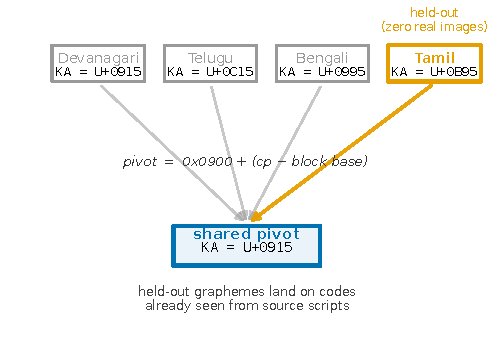
\includegraphics[width=\linewidth]{figs/fig1_pivot.pdf}
  \caption{The shared grapheme pivot space. Each Brahmic script maps bijectively into a common
  output space by ISCII-derived Unicode-offset correspondence (the same letter sits at the same
  offset within each block); grapheme clusters in that space form the recognizer's output
  vocabulary. A held-out script's graphemes therefore land on pivot codes already seen from the
  source scripts. The held-out script enters training only as verified synthetic renderings
  (Rung~B) or not at all (Rung~A); evaluation is always on its \emph{real} scene images.}
  \label{fig:method}
\end{figure}

\subsection{A shared grapheme pivot space for Brahmic scripts}
\label{sec:pivot}

Brahmic scripts encode the same phonological skeleton --- consonant bases, dependent vowel signs,
and conjunct formation through a virama --- and Unicode preserves this: corresponding letters sit
at the same offset within each script's block. We exploit both layers.

\paragraph{Structural pivot.} A mapping $\pi$ sends any Brahmic codepoint to a pivot codepoint by
its within-block offset ($\pi(c) = \mathrm{0x0900} + (c - \mathrm{base}(c))$); shared punctuation
that is not offset-safe is excluded by construction. Because $\pi$ is a per-script bijective
shift, it is exactly invertible: a hypothesis decoded in pivot space is read back into the target
script deterministically. Text from nine scripts thereby writes into one label space in which
structurally corresponding syllables become \emph{identical} strings.

\paragraph{Grapheme-cluster vocabulary.} Within pivot space we segment text into grapheme
clusters (consonant--virama conjuncts kept whole, dependent signs attached) and inject the
resulting cluster inventory (1{,}624 types for the source pool) as dedicated tokens into the
recognizer's tokenizer. The alternative --- letting the stock byte-BPE tokenizer segment
pivot-space text --- is the ablation of Sec.~\ref{sec:experiments}: it sees the same pivot
strings but fragments clusters into sub-syllabic pieces. Fertility (mean clusters per word)
governs when grapheme tokenization beats BPE in \emph{supervised} training: in a 12-run
balanced-budget study across the same nine scripts, fertility predicts the winning branch with
\lawPolarity\ polarity and $\lawLoso\%$ leave-one-script-out direction accuracy
($R^2\!=\!\lawRsqAdv$). % pointer to journal-length treatment; kept to motivation here
That result motivates both the pivot design and the (ultimately falsified) primary hypothesis of
Sec.~\ref{sec:analysis}.

\subsection{Zero-real-image protocol}
\label{sec:protocol}

For each held-out script $S$ of the nine in the benchmark~\cite{bstd}:

\noindent\textbf{Sources.} All benchmark languages whose script is not $S$ (languages sharing
$S$, e.g.\ Assamese for Bengali script, are excluded --- $S$ is genuinely unseen). Each source
language contributes exactly 700 train / 90 val real images (seed 42), giving balanced source
exposure by construction; source-side data size is therefore controlled, unlike prior
cross-lingual STR studies~\cite{crosslingstr}.

\noindent\textbf{Synthetic target.} 3{,}240 images per target language: benchmark-vocabulary
words rendered in fontconfig-verified fonts (multiple faces per script, libraqm shaping), each
render checked non-blank; the rendered word enters training as its pivot transcription. No real
photograph of $S$ is ever seen. Scripts written by two source languages receive two languages'
worth of renderings ($2\times$ budget) --- a covariate disclosed at preregistration time that
becomes central in Sec.~\ref{sec:analysis}.

\noindent\textbf{Rungs.} Rung~A trains on sources only; Rung~B adds the synthetic target set;
Rung~B$_{\mathrm{bpe}}$ repeats Rung~B with the grapheme-cluster injection removed (stock
tokenizer), identical data, seed, and recipe. All rungs fine-tune Florence-2
(0.23B)~\cite{florence2} with LoRA ($r\!=\!16$, $\alpha\!=\!32$, dropout 0.05), lr $10^{-4}$,
batch size 4, 15 epochs, validation-selected checkpoint, beam-search decoding at test.

\noindent\textbf{Evaluation.} The held-out script's real test split, WRR = exact match after NFC
normalization, zero-width-character removal, and whitespace collapse --- the benchmark's own
protocol~\cite{bstd,indicstr12} --- plus character accuracy ($1-\mathrm{CER}$).

\subsection{Preregistration and prospective predictions}
\label{sec:prereg}

The campaign ran under a frozen preregistration with an append-only amendment log; every
amendment was filed before the results it concerns existed. Descriptors entering the transfer
horse-race were computed result-blind: fertility and pivot coverage before any Rung-B result;
a frozen-encoder visual-similarity control before the third. Quantitative forecasts for later
runs were committed and pushed to a version-controlled archive \emph{before} those runs trained
(commit hashes in the supplementary material; archive anonymized for review), and are scored
against a rule fixed at filing time --- hits and misses alike (Sec.~\ref{sec:analysis}).
% Double-blind note: archive cited via anonymous mirror; hashes verifiable at camera-ready.

\section{Experiments}
\label{sec:experiments}

Before any absolute number: supervised recognizers fine-tuned on real labeled target images reach
$\parseqFinetuned\%$ WRR on this benchmark~\cite{bstd}. Those systems answer a different question
--- they presuppose the labeled data whose absence defines our setting. The comparisons that
match our question are: the source-only baseline (Rung~A), the raw pre-trained VLM (WRR
$\florenceRawZS$), the stock-BPE ablation, frontier VLMs prompted zero-shot on the same test
sets, and our own forecasts.

\subsection{Main result: every unseen script becomes readable}
\label{sec:mainresult}

\begin{table}[t]
  \centering\small
  \setlength{\tabcolsep}{2.7pt}
  \begin{tabular}{lrrrcrr}
    \toprule
    Script & $N$ & A & B & \footnotesize B 95\% CI & CharAcc & B$_{\mathrm{bpe}}$ \\
    \midrule
    Tamil      & \ntamil      & \wrrAtamil      & \textbf{\wrrBtamil}      & {\footnotesize\ciBtamil}      & \chaBtamil      & \wrrPtamil \\
    Telugu     & \ntelugu     & \wrrAtelugu     & \textbf{\wrrBtelugu}     & {\footnotesize\ciBtelugu}     & \chaBtelugu     & \wrrPtelugu \\
    Kannada    & \nkannada    & \wrrAkannada    & \textbf{\wrrBkannada}    & {\footnotesize\ciBkannada}    & \chaBkannada    & \wrrPkannada \\
    Malayalam  & \nmalayalam  & \wrrAmalayalam  & \textbf{\wrrBmalayalam}  & {\footnotesize\ciBmalayalam}  & \chaBmalayalam  & \wrrPmalayalam \\
    Oriya      & \noriya      & \wrrAoriya      & \textbf{\wrrBoriya}      & {\footnotesize\ciBoriya}      & \chaBoriya      & \wrrPoriya \\
    Gujarati   & \ngujarati   & \wrrAgujarati   & \textbf{\wrrBgujarati}   & {\footnotesize\ciBgujarati}   & \chaBgujarati   & \wrrPgujarati \\
    Bengali    & \nbengali    & \wrrAbengali    & \textbf{\wrrBbengali}    & {\footnotesize\ciBbengali}    & \chaBbengali    & \wrrPbengali \\
    Devanagari & \ndevanagari & \wrrAdevanagari & \textbf{\wrrBdevanagari} & {\footnotesize\ciBdevanagari} & \chaBdevanagari & \wrrPdevanagari \\
    Gurmukhi   & \ngurmukhi   & \wrrAgurmukhi   & \textbf{\wrrBgurmukhi}   & {\footnotesize\ciBgurmukhi}   & \chaBgurmukhi   & \wrrPgurmukhi \\
    \bottomrule
  \end{tabular}
  \caption{Zero-real-image transfer across nine held-out Brahmic scripts (real test images).
  Rung~A: source scripts only. Rung~B: + synthetic target renderings, zero real target images
  (95\% CI = percentile bootstrap over test samples, 5000 resamples). B$_{\mathrm{bpe}}$: Rung~B
  with the grapheme-cluster vocabulary removed (stock tokenizer), identical data and seed. On
  \bpeCIdisjoint/9 scripts the Rung-B CI lies strictly above the B$_{\mathrm{bpe}}$ point.}
  \label{tab:main}
\end{table}

Table~\ref{tab:main} is the campaign's core. Every one of the nine scripts moves from a
near-floor source-only baseline (\wrrAtamil--\wrrAdevanagari\% WRR; the raw pre-trained model
reads none of them) to \wrrBmin--\wrrBmax\% WRR with character accuracy \chaBmalayalam--%
\chaBbengali\% --- without a single real target image. Transfer does not collapse even on the
hardest script (Malayalam, lowest pivot coverage at \covmalayalam\%: still
$\wrrAmalayalam\!\rightarrow\!\wrrBmalayalam$). Rung-A baselines track incidental pivot-space
coverage (highest for Devanagari, \wrrAdevanagari\%), confirming the pivot shares structure
before any target exposure.

% Fig 2: grouped bars A/B/Bbpe per script
\begin{figure}[t]
  \centering
  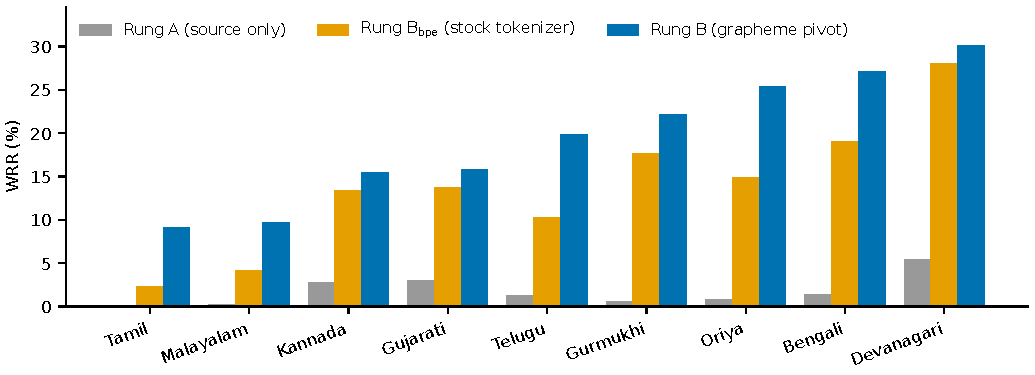
\includegraphics[width=\linewidth]{figs/fig2_bars.pdf}
  \caption{Transfer by script (ascending by Rung~B). Source-only baselines (grey) sit near the
  floor; the grapheme pivot (blue) beats the stock-BPE tokenizer (orange) on every one of the nine
  scripts under identical data and seed. Generated from the result JSONs by
  \texttt{make\_wacv\_figs.py}.}
  \label{fig:bars}
\end{figure}

\subsection{The pivot is the mechanism: BPE ablation}
\label{sec:ablation}

Removing the grapheme-cluster vocabulary --- same pivot strings, same images, same seed ---
degrades all nine scripts (Table~\ref{tab:main}), from $\bpeRatioMin\times$ (Devanagari,
\wrrBdevanagari\ $\rightarrow$ \wrrPdevanagari\ WRR) to $\bpeRatioMax\times$ (Tamil,
\wrrBtamil\ $\rightarrow$ \wrrPtamil): the margin varies, the direction never does (exact
two-sided sign test, $p=\bpeSignP$). The bootstrap makes the per-script margin concrete: on
\bpeCIdisjoint\ of nine the Rung-B 95\% CI clears the B$_{\mathrm{bpe}}$ interval outright
(Table~\ref{tab:main}); the three exceptions --- Devanagari, Kannada, Gujarati --- are exactly the
near-parity scripts ($\bpeRatioMin$--$1.16\times$), consistent with the direction holding but the
magnitude shrinking as fertility falls. The character-accuracy pattern is diagnostic: on Telugu
the BPE model \emph{matches} the pivot model's character accuracy (\chaPtelugu\% vs.\
\chaBtelugu\%), and on Kannada and Devanagari slightly exceeds it, yet word accuracy drops in
every case. Synthetic fine-tuning alone teaches the model to see the characters; the
cluster-level output space is what assembles them into correct whole words. The margin itself
is not noise: it grows with the held-out script's fertility, largest exactly on the
high-fertility Dravidian scripts where transfer is hardest
(Sec.~\ref{sec:fertility-fails}).

\subsection{Dose--response: synthetic budget}
\label{sec:scaling}

We hold the recipe fixed and vary only the number of synthetic target images, for the three
scripts whose held-out budget we can grow --- Malayalam, Kannada, Telugu --- across
$\{810, 1620, 6480, 12960\}$ renderings; the external Rung-B point (3240) anchors each curve.
Word recognition is cleanly log-linear in synthetic exposure ($R^2$ from \scaleRtwoMin\ to
\scaleRtwoMax\ per script), and the slope is \emph{script-invariant}: a single shared
$\scaleSlope$ WRR per doubling fits all three, with no evidence of differing slopes ($F$-test
$p=\scaleFp$; Fig.~\ref{fig:scaling}). This is the preregistered \emph{form}, and it holds.

The preregistered \emph{magnitude} does not. The frozen instrument projected
$+\tfTwoxBonus$ WRR per doubling --- transported from the in-script $2\times$-synthetic experiment
that fit the two-factor model (Sec.~\ref{sec:analysis}) --- which the swept slope excludes by a
factor of $\scaleSlopeRatio$: the faithful doubling step ($3240\!\rightarrow\!6480$) gained
$\scaleFaithfulObs$ WRR on average against a predicted $\scaleFaithfulPred$, a miss outside the
$\pm2$\,RMSE band and reported as filed (open squares, Fig.~\ref{fig:scaling}). Two further
preregistered edges resolve the same way. The low-budget prediction of near-collapse toward the
Rung-A floor is \emph{falsified} --- Kannada and Telugu already reach double digits at 810 images,
so transfer is concave, not linear, in log-budget --- while the top step
($6480\!\rightarrow\!12960$), which adds renderings at near-fixed lexicon, gains little on Kannada
(onset of lexicon saturation) but keeps pace on Malayalam and Telugu. Synthetic scaling is thus
real and orderly, but far shallower than an in-script extrapolation predicts; we report the
confirmed form and the missed coefficient together. We do \emph{not} promote pivot-space coverage
to a cross-script driver: it orders the three swept scripts in-sample, but across the six scripts
never used in the fit it is uncorrelated with transfer ($r=\covOOSr$), so the coverage axis (three
distinct values) is underdetermined and we disclose it rather than build on it.

\begin{figure}[t]
  \centering
  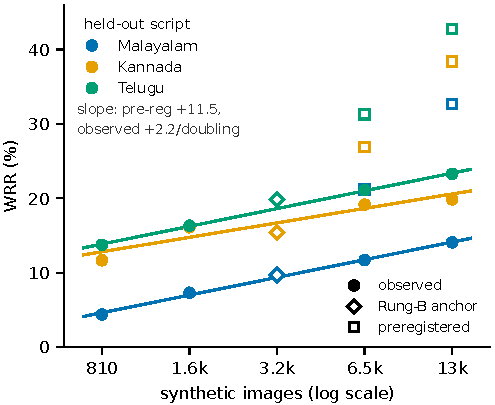
\includegraphics{figs/fig3_scaling.pdf}
  \caption{Synthetic-budget dose--response for three held-out scripts. Filled circles: observed WRR
  on real test images; solid lines: per-script log-linear fits (shared slope
  $\scaleSlope$/doubling). Open diamonds: the external Rung-B anchor (3240 images). Open squares:
  the preregistered point predictions --- their gap above the observed points is the
  $\scaleSlopeRatio\times$ magnitude miss, reported as filed.}
  \label{fig:scaling}
\end{figure}

\subsection{Out-of-benchmark: Khmer}
\label{sec:khmer}

\TODO{Preregistered Amendment 4b: train on all nine benchmark scripts + synthetic Khmer
(different Unicode block, coeng-based stacking, outside the benchmark and outside India);
evaluate on KhmerST~\cite{khmerst}. PROSPECTIVE\_PREDICTION\_KHMER filed from the frozen
two-factor model before training. Timeboxed; paper stands without it if the segmenter/crop
engineering misses the freeze date.}

\subsection{Frontier-VLM reference}
\label{sec:vlm}

We prompt Qwen2.5-VL-7B~\cite{qwen25vl} zero-shot on the same nine real test sets (fixed prompt,
greedy decoding), preregistered under Amendment~4c. Under the declared primary metric --- exact
word match on the raw generation, our shared normalization --- it scores $0.0\%$ on all nine: the
chat model wraps every answer in prose (``The text in the image is~\dots''). We therefore report a
\emph{disclosed, most-favourable} re-score (Table~\ref{tab:vlm}): we extract the first quoted span
from each generation and apply the identical metric. Even so, the VLM reads only the two
highest-resource scripts with any competence --- Bengali \vlmWrrBengali\% and Devanagari
\vlmWrrDevanagari\% --- and is at or near zero on six of the remaining seven (at most
\vlmWrrTamil\%, on Tamil), frequently transcribing a wholly different script (Gurmukhi returned in
Devanagari, Malayalam in Bengali). Our compact pivot model, at a fraction of the parameters, wins
on \vlmScriptsWon\ of nine, the VLM leading only on Devanagari, the single most-resourced Indic
script. The comparison is not like-for-like --- the VLM's training data is unknown and it is an
upper-bound reference for off-the-shelf capability, not a system built for this task --- but it
establishes that scale alone does not read these scripts; frontier models cover fewer than thirty
of 100+ writing systems~\cite{glotocr}.

\begin{table}[t]
  \centering\small
  \setlength{\tabcolsep}{6pt}
  \begin{tabular}{lrr}
    \toprule
    Script & Ours (Rung~B) & Qwen2.5-VL-7B \\
    \midrule
    Tamil      & \textbf{\wrrBtamil}      & \vlmWrrTamil      \\
    Telugu     & \textbf{\wrrBtelugu}     & \vlmWrrTelugu     \\
    Kannada    & \textbf{\wrrBkannada}    & \vlmWrrKannada    \\
    Malayalam  & \textbf{\wrrBmalayalam}  & \vlmWrrMalayalam  \\
    Oriya      & \textbf{\wrrBoriya}      & \vlmWrrOriya      \\
    Gujarati   & \textbf{\wrrBgujarati}   & \vlmWrrGujarati   \\
    Bengali    & \textbf{\wrrBbengali}    & \vlmWrrBengali    \\
    Devanagari & \wrrBdevanagari          & \textbf{\vlmWrrDevanagari} \\
    Gurmukhi   & \textbf{\wrrBgurmukhi}   & \vlmWrrGurmukhi   \\
    \midrule
    macro avg  & --                       & \vlmMacro         \\
    \bottomrule
  \end{tabular}
  \caption{Zero-shot WRR (\%) vs.\ a frontier VLM on the same real test images. Qwen2.5-VL scored
  under a disclosed, most-favourable extraction (its preregistered exact-match primary is $0.0$ on
  all nine). Our compact model wins on \vlmScriptsWon\ of nine; the VLM leads only on Devanagari,
  the most-resourced Indic script.}
  \label{tab:vlm}
\end{table}

\section{What Predicts Transfer?}
\label{sec:analysis}

We report the confirmatory analysis exactly as preregistered, our own primary hypothesis included.

\begin{figure}[t]
  \centering
  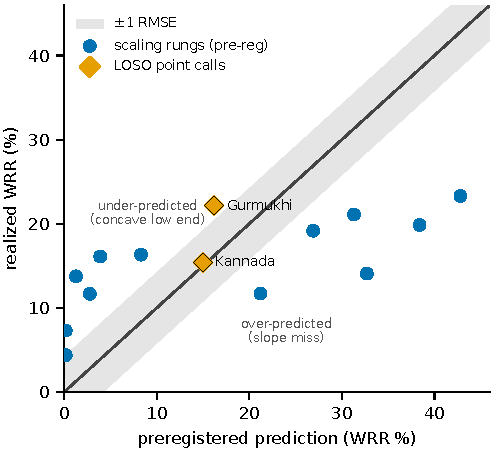
\includegraphics[width=\linewidth]{figs/fig4_receipts.pdf}
  \caption{Prospective scorecard: preregistered prediction vs.\ realized WRR for every quantitative
  forecast filed before its run, scored against the rule fixed at filing time (shaded $\pm1$ RMSE).
  The in-block LOSO point calls land on the diagonal; the scaling rungs fall off it both ways ---
  under-predicted at low budget, over-predicted at high. Khmer, the out-of-block call, misses low by
  $\khmerResidRMSE\cdot$RMSE. Hits and misses are both shown.}
  \label{fig:receipts}
\end{figure}

\subsection{The preregistered primary fails}
\label{sec:fertility-fails}

Fertility, the property that governs the supervised grapheme-vs-BPE trade-off
(Sec.~\ref{sec:pivot}), was preregistered as the primary transfer predictor (H3). It is
refuted: Spearman $\rho=\spearFert$ across the nine Rung-B results, directionally
\emph{opposite} to the hypothesis. The flagship case was called in advance by the declared
competitor: our prospective prediction file ranked Malayalam best under fertility (P1) and worst
under coverage (P2); it realized bottom-tier (\wrrBmalayalam\ WRR). We report this as a genuine
falsification, consistent with fertility skepticism in the LLM-tokenizer
literature~\cite{beyondfertility} and with the data-centric view of STR
transfer~\cite{crosslingstr}.

Post-hoc, fertility instead tracks \emph{who needs the pivot}: BPE comes closest to parity on the
lowest-fertility script and collapses on the highest ($\bpeRatioMin\times$ Devanagari,
$\bpeRatioMax\times$ Tamil). That is unregistered, $n=9$, and used for nothing here.

\subsection{The two-factor account}
\label{sec:twofactor}

Two result-blind quantities describe the campaign and generated its forecasts; we state them as
description, not inference, because at $n=9$ scripts nothing here carries appreciable inferential
force. Synthetic budget dominates: the two scripts with the disclosed $2\times$ budget (Bengali,
Devanagari) are the top two results (\wrrBbengali, \wrrBdevanagari\ WRR), Bengali from the
second-\emph{lowest} coverage. Coverage orders the seven equal-budget scripts
($\rho=\spearCovEqual$). The joint fit
$\mathrm{WRR} = \tfIntercept + \tfCovCoef\cdot\mathrm{cov} + \tfTwoxBonus\cdot\mathbb{1}[2\times]$
(RMSE \tfRMSE\ WRR) is the instrument every later forecast was drawn from, so we print it for
audit, and then discount it ourselves: a script-level bootstrap puts its coverage slope at
\ciTfCov, \emph{spanning zero}, and that term fails out-of-sample outright ($r=\covOOSr$,
Sec.~\ref{sec:scaling}). Coverage is an in-sample ordering and nothing more. One control stands on
its own: rendered glyphs embedded by the recognizer's own frozen vision encoder predict transfer
not at all ($\rho=\spearVissim$), separating whatever the ordering reflects from the
visual-similarity account of~\cite{crosslingstr}.

\subsection{Prospective scorecard}
\label{sec:scorecard}

Four forecasts were filed before their runs and all four are scored in
Fig.~\ref{fig:receipts}. Two are in-block point calls: \textbf{Kannada} ($\predKannada$ WRR, filed
with two scripts observed, realized \realKannada) and \textbf{Gurmukhi}, the final script
(\predGurmukhi\ WRR with $\pm1\sigma$ \predGurmukhiOneSig, committed \emph{and pushed} 3.7 hours
before training began, realized \realGurmukhi, under-called by $\gurmukhiSigma\sigma$ but inside
$\pm2\sigma$). A third, \textbf{Devanagari}, was a directional call committed before the result
existed but pushed after; it is only weakly prospective and we lean on it for nothing. The fourth
is \textbf{Khmer} (Sec.~\ref{sec:khmer}), the one call filed outside the pivot's Unicode blocks,
which missed by $\khmerResidRMSE\sigma$. The declared rank bet between the two preregistered
predictors resolved for coverage over fertility, neither ranking alone significant at $n=7$.

The summary is bounded: in-block, transfer is forecastable to roughly $\pm\tfRMSE$ WRR
($1\sigma$) from two pre-training quantities, but the instrument missed out of block and we decline
to extend it past the blocks it was fit on: one script shows it failed there, not that it must
fail everywhere outside.

\section{Limitations}
\label{sec:limitations}

\textbf{Absolute accuracy.} \wrrBmin--\wrrBmax\% WRR clears an off-the-shelf per-script OCR floor
(\tessMean\%) but remains far below the supervised ceiling ($\parseqFinetuned\%$ with real labeled
data~\cite{bstd}); the synthetic $\rightarrow$ real domain gap is the dominant residual, quantified
by training loss reaching ${\sim}0.06$ on synthetic data while real-image WRR stays modest.
\textbf{One family, and a located boundary.} Nine scripts, one benchmark, one family whose shared
structure the pivot exploits by design. Khmer (Sec.~\ref{sec:khmer}) does not merely leave
non-Brahmic generalization open --- it shows the method \emph{failing} there (\khmerB\% WRR), and
we make no claim beyond the family. \textbf{One architecture.} All transfer results use
Florence-2; a from-scratch CRNN replicates the direction but at ${\sim}\crnnRatioMean$ of the
magnitude (Sec.~\ref{sec:crnn}), so backbone-independence of the effect size is untested.
\textbf{Model imperfections.} Gujarati underperforms its coverage, one Rung-A baseline breaches
the predicted $<5$ line by 0.46 (Devanagari, \wrrAdevanagari), and the final-script forecast
under-called by $1.5\sigma$; all reported, none explained away. \textbf{Compute.} Single 24\,GB
GPU; budgets (700/source, 3{,}240 synthetic) were fixed by preregistration, not tuned.

\section{Conclusion}
\label{sec:conclusion}

We showed that real scene text of an entirely unseen Brahmic script can be read --- at
\wrrBmin--\wrrBmax\% word accuracy across all nine scripts of a public benchmark, ahead of stock
per-script Tesseract on \tessScriptsWon\ of nine despite never seeing a real image of the target
--- by a small open VLM fine-tuned in a shared grapheme pivot space with only rendered synthetic
exposure, and that a stock-BPE ablation collapses this transfer, isolating output-space structure
as the mechanism. The campaign ran under a frozen preregistration, and its forecasting record is
mostly a record of misses: the primary hypothesis falsified, the scaling magnitude missed by
$\scaleSlopeRatio\times$, coverage failing out-of-sample, and the one out-of-block forecast (Khmer)
missed by $\khmerResidRMSE\sigma$. We advance no predictive law; every call is auditable by commit
hash, and the failures locate the method's boundary rather than leaving it for someone else to
find. Beyond the specific results we offer the recipe --- structural pivot, verified rendering,
forecast-before-you-run --- as a template for the long tail.

{
    \small
    \bibliographystyle{ieeenat_fullname}
    \bibliography{main}
}

\end{document}
